\section{Ejercicio \#3: Algoritmo Aspiradora Robot}

\subsection{Introducción y Problema}

En este ejercicio se modela el recorrido de una aspiradora robot dentro de un laberinto rectangular. El laberinto se representa mediante una matriz,
donde cada celda puede corresponder a una pared (\textit{X}), una posición transitable, la entrada (\textit{E}) o la salida (\textit{S}).

El objetivo es diseñar, implementar y documentar un algoritmo de backtracking que, dado un laberinto de tamaño $m \times n$, encuentre un camino
válido desde la posición inicial \textit{E} hasta la salida \textit{S}, en caso de que dicho camino exista.

La solución devuelve el recorrido como una secuencia de coordenadas de la matriz. A partir de ese camino, pueden interpretarse
los movimientos que debería realizar la aspiradora para desplazarse por el laberinto, utilizando sus operaciones disponibles:
observar la celda siguiente, avanzar y girar.

\subsection{Algoritmo de Backtracking}

El problema se resuelve mediante backtracking. Desde la entrada \textit{E}, el algoritmo intenta avanzar recursivamente hacia las posiciones vecinas en un orden fijo: derecha, izquierda, abajo y arriba.

Antes de avanzar, se verifica que la celda esté dentro de los límites, que no sea una pared \textit{X} y que no haya sido visitada previamente. Si la celda es válida, se agrega a la solución y se marca como visitada.

Cuando se alcanza la salida \textit{S}, se devuelve el camino encontrado. Si desde una posición no se puede continuar hacia la salida, se elimina esa posición de la solución y se vuelve atrás para probar otra alternativa.

\subsection{Supuestos}

Se asume que el laberinto es rectangular, por lo que todas sus filas tienen la misma cantidad de columnas. Sus dimensiones se obtienen a partir del archivo de entrada.

También se asume que existe una única posición inicial \textit{E} y al menos una salida \textit{S}. Las celdas marcadas con \textit{X} representan paredes y no pueden ser recorridas. Del mismo modo, cualquier posición fuera de los límites del laberinto se considera inválida.

En caso de que no exista un camino posible entre la entrada y la salida, el algoritmo devuelve una lista vacía.

\subsection{Diseño}

La solución se basa en un algoritmo recursivo de backtracking. En cada llamada se analiza una posición del laberinto y se verifica si puede ser recorrida. Una posición es válida si está dentro de los límites de la matriz, no corresponde a una pared y no fue visitada anteriormente.

Si la posición es válida, se agrega a la solución y se marca como visitada. Luego se prueban las cuatro direcciones posibles en un orden fijo: derecha, izquierda, abajo y arriba. Si alguna de esas ramas alcanza la salida, el algoritmo termina y devuelve el camino encontrado. En caso contrario, se elimina la posición actual de la solución y se retrocede para probar otras alternativas.

Las estructuras de datos utilizadas son:

\begin{itemize}
    \item Una matriz de caracteres para representar el laberinto.
    \item Una lista con la solución construida hasta el momento.
    \item Un conjunto de posiciones visitadas para evitar ciclos y no recorrer dos veces la misma celda.
\end{itemize}

A continuación se presenta el pseudocódigo del algoritmo:

\lstinputlisting[]{code/laberinto.txt}

\subsection{Podas}

El algoritmo aplica dos podas que reducen el espacio de búsqueda:

\begin{itemize}
    \item \textbf{Posición inválida}: antes de explorar una celda se verifica que esté dentro de los límites del laberinto y que no sea una pared. Si alguna de estas condiciones no se cumple, la rama se descarta de inmediato sin continuar la recursión.
    \item \textbf{Conjunto de visitados}: cada celda que se incorpora a la solución se registra en un conjunto. Si una dirección conduce a una celda ya visitada, esa rama se descarta sin explorarla. Esta poda elimina ciclos e impide recorrer la misma celda más de una vez, garantizando que el árbol de búsqueda sea finito.
\end{itemize}

\subsection{Ejecución}

El código se encuentra en \textit{ejercicios/ej-backtracking/}. Para ejecutar el algoritmo sobre un archivo de entrada:

\begin{verbatim}
python ejercicios/ej-backtracking/laberinto.py <archivo_input>
\end{verbatim}

Para correr todos los casos de prueba contra los resultados esperados:

\begin{verbatim}
python ejercicios/ej-backtracking/run_all_tests.py
\end{verbatim}

\subsection{Seguimiento}

Para el seguimiento se utiliza el siguiente laberinto de $5 \times 5$, donde \textit{E} se encuentra en la posición $(1,1)$ y \textit{S} en la posición $(3,3)$ (índices base cero). Las celdas libres se indican con \textbf{·}.

\begin{center}
\begin{tabular}{|c|c|c|c|c|}
\hline
X & X & X & X & X \\
\hline
X & E & $\cdot$ & $\cdot$ & X \\
\hline
X & $\cdot$ & X & X & X \\
\hline
X & $\cdot$ & $\cdot$ & S & X \\
\hline
X & X & X & X & X \\
\hline
\end{tabular}
\end{center}

El orden de exploración de direcciones es: derecha, izquierda, abajo, arriba.

\begin{center}
\begin{tabular}{|c|l|l|}
\hline
\textbf{Paso} & \textbf{Llamada / acción} & \textbf{Solución} \\
\hline
1  & \texttt{avanzar(1,1)}: válida, agregar               & \texttt{[(1, 1)]} \\
2  & \texttt{avanzar(1,2)}: válida, agregar               & \texttt{[(1, 1), (1, 2)]} \\
3  & \texttt{avanzar(1,3)}: válida, agregar               & \texttt{[(1, 1), (1, 2), (1, 3)]} \\
4  & \texttt{avanzar(1,4)}: pared $\rightarrow$ FALSO     & — \\
5  & \texttt{avanzar(1,2)}: visitada $\rightarrow$ FALSO  & — \\
6  & \texttt{avanzar(2,3)}: pared $\rightarrow$ FALSO     & — \\
7  & \texttt{avanzar(0,3)}: pared $\rightarrow$ FALSO     & — \\
8  & \textbf{BACKTRACK}: sin salida desde (1,3), quitar   & \texttt{[(1, 1), (1, 2)]} \\
9  & \texttt{avanzar(1,1)}: visitada $\rightarrow$ FALSO  & — \\
10 & \texttt{avanzar(2,2)}: pared $\rightarrow$ FALSO     & — \\
11 & \texttt{avanzar(0,2)}: pared $\rightarrow$ FALSO     & — \\
12 & \textbf{BACKTRACK}: sin salida desde (1,2), quitar   & \texttt{[(1, 1)]} \\
13 & \texttt{avanzar(1,0)}: pared $\rightarrow$ FALSO     & — \\
14 & \texttt{avanzar(2,1)}: válida, agregar               & \texttt{[(1, 1), (2, 1)]} \\
15 & \texttt{avanzar(2,2)}: pared $\rightarrow$ FALSO     & — \\
16 & \texttt{avanzar(2,0)}: pared $\rightarrow$ FALSO     & — \\
17 & \texttt{avanzar(3,1)}: válida, agregar               & \texttt{[(1, 1), (2, 1), (3, 1)]} \\
18 & \texttt{avanzar(3,2)}: válida, agregar               & \texttt{[(1, 1), (2, 1), (3, 1), (3, 2)]} \\
19 & \texttt{avanzar(3,3)}: salida \textit{S} $\rightarrow$ VERDADERO & \texttt{[(1, 1), (2, 1), (3, 1), (3, 2), (3, 3)]} \\
\hline
\end{tabular}
\end{center}

El algoritmo primero explora hacia la derecha, llegando a $(1,3)$ sin poder continuar. Al no encontrar salida, retrocede (pasos 8 y 12) hasta $(1,1)$ y prueba la dirección abajo. Desde allí encuentra el camino correcto sin nuevos retrocesos.

El camino devuelto es:

\begin{verbatim}
[(1, 1), (2, 1), (3, 1), (3, 2), (3, 3)]
\end{verbatim}

\subsection{Resultados experimentales}

Para validar el comportamiento del algoritmo, se ejecutó la solución sobre cinco conjuntos de datos con laberintos de distinto tamaño. En todos los casos, el algoritmo finalizó correctamente y devolvió un camino válido desde la entrada \textit{E} hasta la salida \textit{S}. Para las mediciones se utilizó el módulo \textit{ejercicios/ej-backtracking/run\_all\_tests.py}, que imprime el tiempo de ejecución.

Los tiempos de ejecución obtenidos fueron los siguientes:

\begin{center}
\begin{tabular}{|c|c|}
\hline
Caso & Tiempo de ejecución \\
\hline
Laberinto 1 & $79.209$ $\mu$s \\
Laberinto 2 & $88.500$ $\mu$s \\
Laberinto 3 & $117.834$ $\mu$s \\
Laberinto 4 & $172.042$ $\mu$s \\
Laberinto 5 & $202.000$ $\mu$s \\
\hline
\end{tabular}
\end{center}

A continuación se presenta un gráfico comparativo de los tiempos medidos para cada conjunto de datos.

\begin{center}
    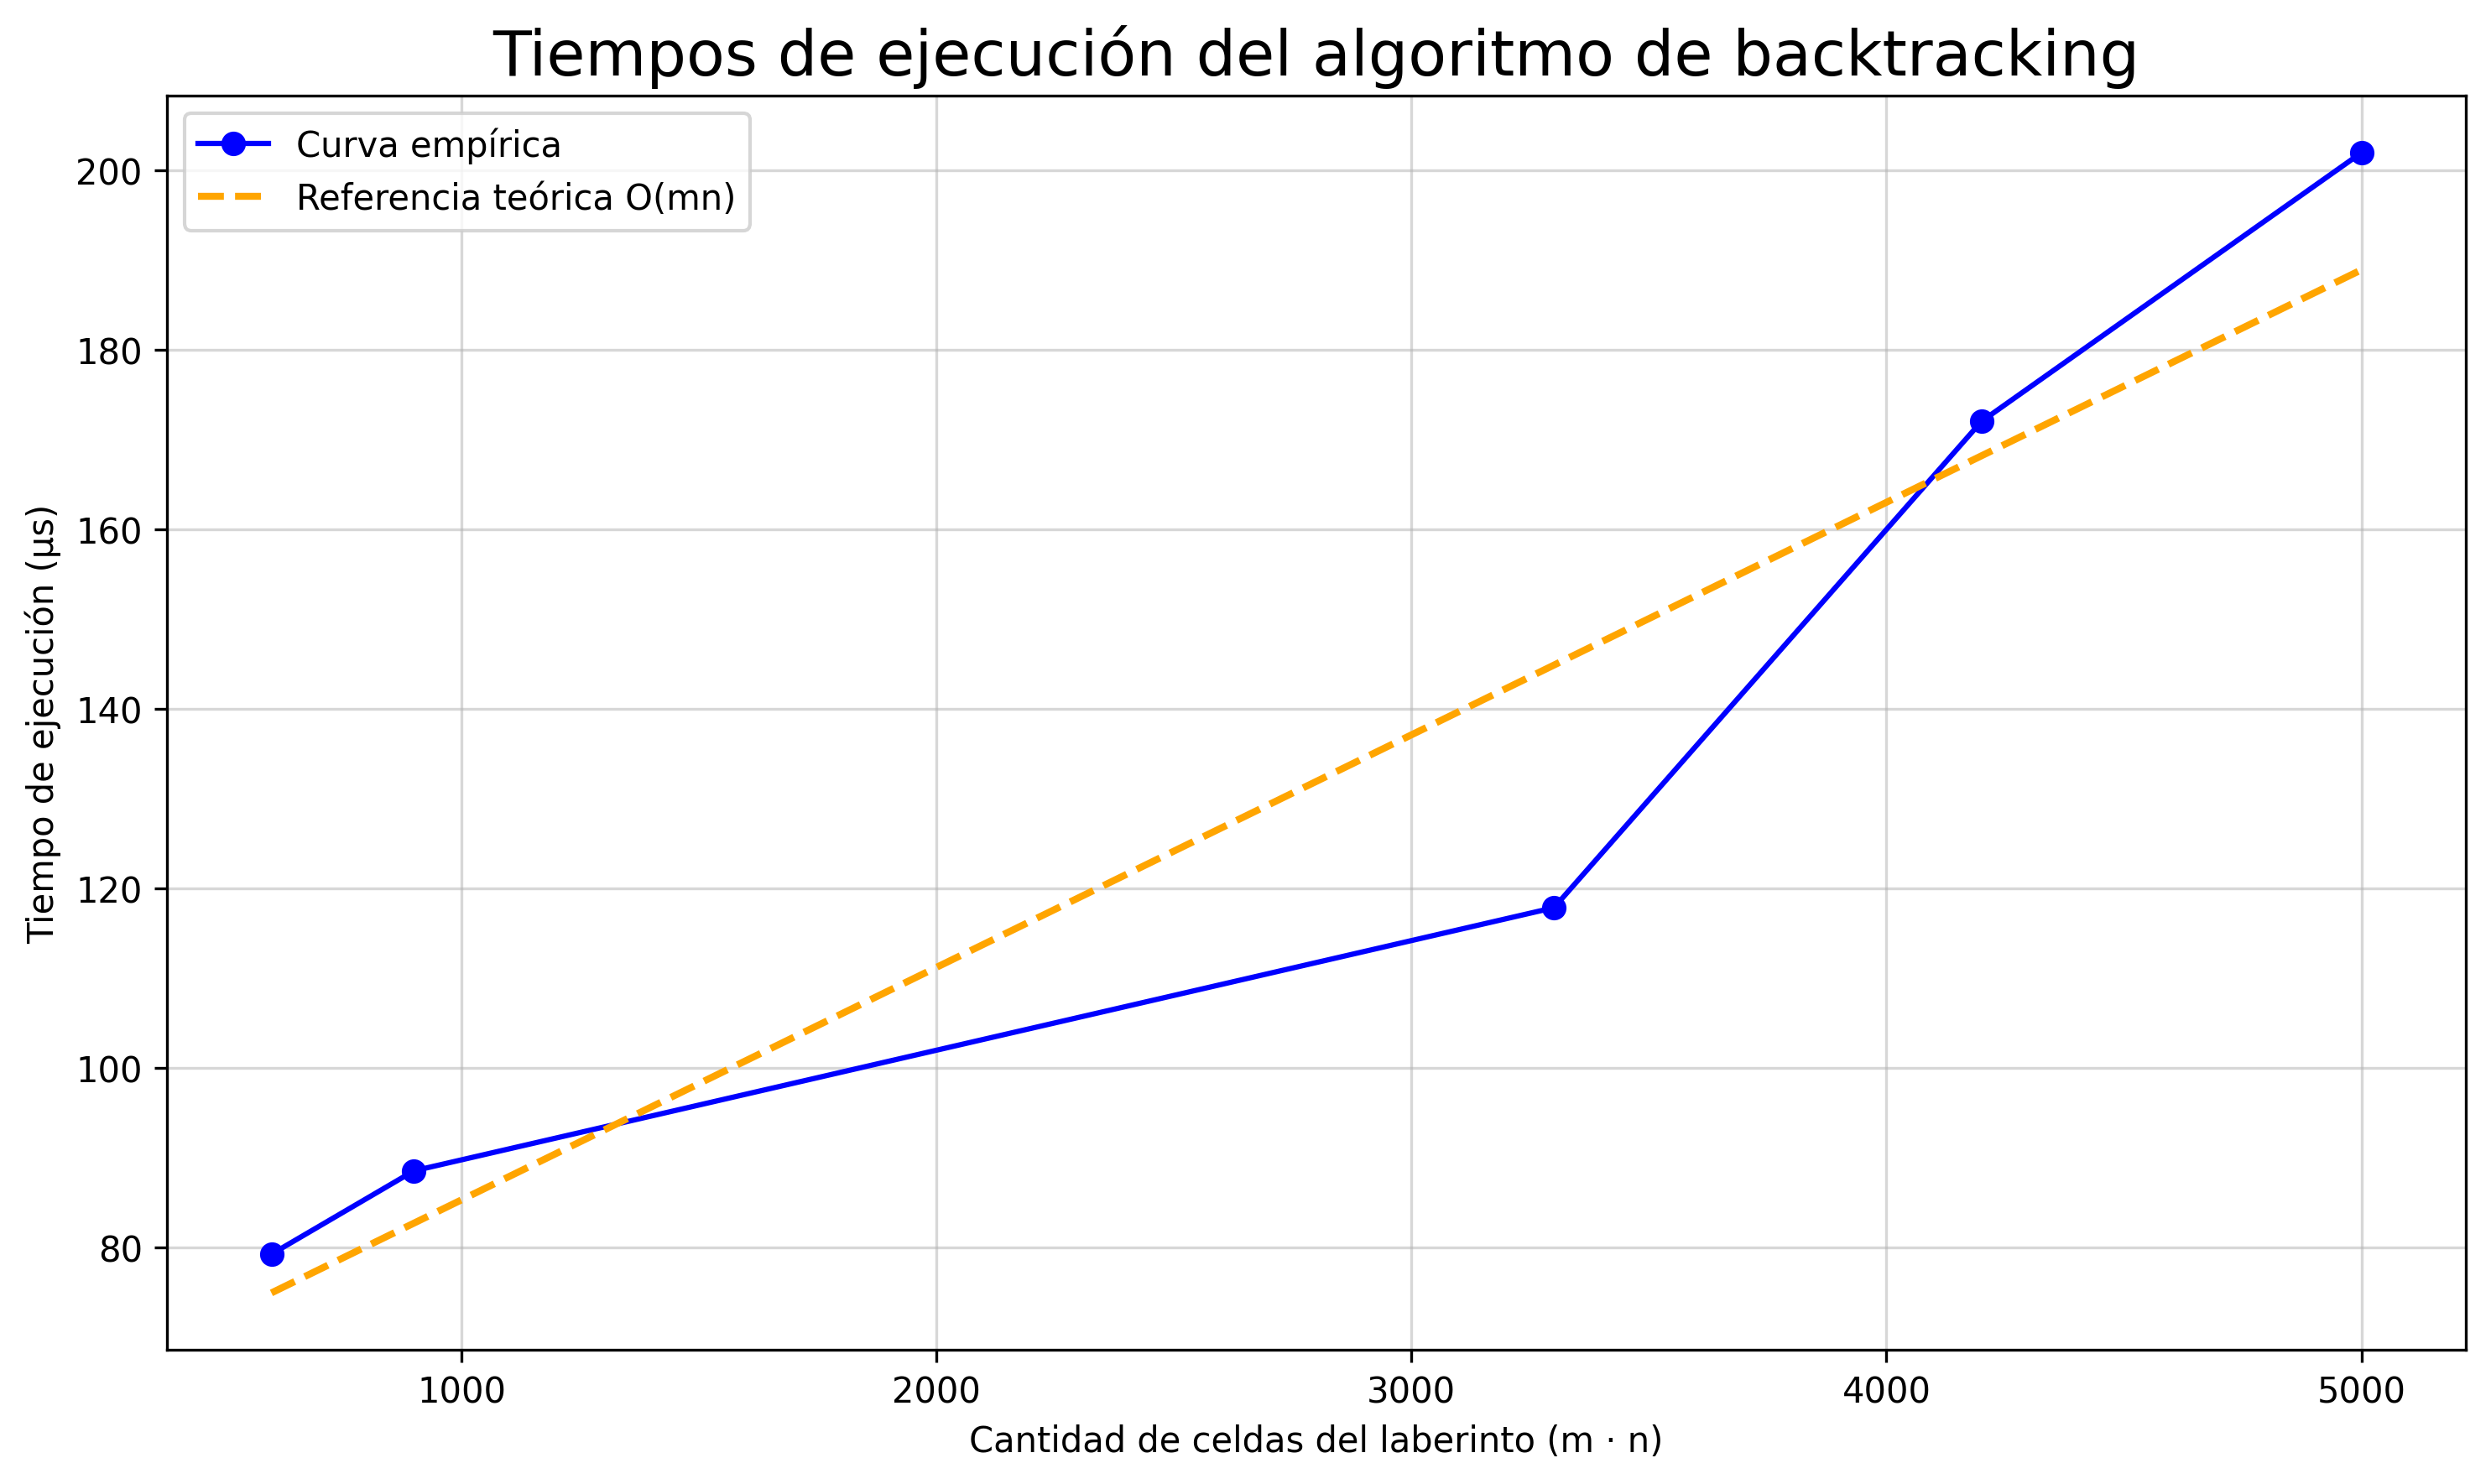
\includegraphics[width=0.75\textwidth]{img/ej3_tiempos.png}
\end{center}

Como se observa en la tabla y en el gráfico, los tiempos de ejecución presentan una tendencia creciente a medida que aumenta el tamaño de los laberintos. Esto resulta coherente con el análisis teórico, ya que para entradas más grandes el algoritmo puede requerir explorar una mayor cantidad de posiciones antes de encontrar la salida.

\subsection{Complejidad temporal y espacial}

Sea $m$ la cantidad de filas del laberinto y $n$ la cantidad de columnas. En el peor caso, el algoritmo puede llegar a analizar todas las celdas de la matriz.

Como las posiciones visitadas se almacenan en un conjunto, cada celda se analiza a lo sumo una vez y la consulta para saber si ya fue visitada tiene costo promedio $O(1)$. Para cada posición válida se prueban hasta cuatro direcciones posibles: derecha, izquierda, abajo y arriba. Como la cantidad de direcciones es constante, la complejidad temporal resulta:

\[
O(mn)
\]

La complejidad espacial también es $O(mn)$. Esto se debe a que el algoritmo almacena la solución y el conjunto de posiciones visitadas. En el peor caso, ambas estructuras pueden crecer proporcionalmente a la cantidad total de celdas del laberinto.

Por lo tanto, tanto la complejidad temporal como la espacial del algoritmo son $O(mn)$.

\subsection{Relación con los resultados}

Los tiempos medidos son bajos, por lo que pueden verse afectados en parte por factores propios de la ejecución y de la medición. Sin embargo, al considerar los cinco conjuntos de datos, se observa una tendencia creciente a medida que aumenta el tamaño del laberinto.

Estos resultados son compatibles con la complejidad temporal, $O(mn)$, ya que el algoritmo recorre como máximo una vez cada celda del laberinto y, para cada una, prueba una cantidad constante de direcciones.

De todos modos, el tiempo de ejecución no depende únicamente de la cantidad total de celdas, sino también de la distribución de paredes y de la ubicación de la salida. Si la salida se encuentra rápidamente, el algoritmo puede finalizar sin recorrer toda la matriz. En cambio, si el camino requiere explorar más alternativas, el tiempo aumenta.

Por lo tanto, los resultados experimentales acompañan el análisis teórico: en los casos evaluados, al aumentar el tamaño del laberinto también aumenta el tiempo de ejecución, manteniéndose dentro del comportamiento esperado para una búsqueda con backtracking sobre una matriz.
